%% $RCSfile: proj_report_outline.tex,v $
%% $Revision: 1.3 $
%% $Date: 2016/06/10 03:41:54 $
%% $Author: kevin $




\documentclass[11pt
              , a4paper
              , twoside
              , openright
              ]{report}


\usepackage{pdfpages}
\usepackage{amsmath}
\usepackage{amssymb}
\usepackage{graphicx}
\usepackage{bm}
\usepackage{subcaption}
\usepackage{float} % lets you have non-floating floats
\usepackage{booktabs}
\usepackage{url} % for typesetting urls
%
%  We don't want figures to float so we define
%
\newfloat{fig}{thp}{lof}[chapter]
\floatname{fig}{Figure}

%% These are standard LaTeX definitions for the document
%%                            
\title{Bayesian estimation of bound fluid fraction from NMR relaxation \\ Preliminary Report}
\author{David Dobbie}

%% This file can be used for creating a wide range of reports
%%  across various Schools
%%
%% Set up some things, mostly for the front page, for your specific document
%
% Current options are:
% [ecs|msor|sms]          Which school you are in.
%                         (msor option retained for reproducing old data)
% [bschonscomp|mcompsci]  Which degree you are doing
%                          You can also specify any other degree by name
%                          (see below)
% [font|image]            Use a font or an image for the VUW logo
%                          The font option will only work on ECS systems
%
\usepackage[image,ecs,]{vuwproject}
\usepackage[a4paper, total={6.5in, 10in}]{geometry}
% You should specifiy your supervisor here with
     \supervisors{Paul Teal, Robin Dykstra}
% use \supervisors if there is more than one supervisor

% Unless you've used the bschonscomp or mcompsci
%  options above use
   \otherdegree{Bachelor of Engineering with Honours in Electronic and Computer Systems Engineering}
% here to specify degree

% Comment this out if you want the date printed.
\date{}

\begin{document}

% Make the page numbering roman, until after the contents, etc.
\frontmatter

%%%%%%%%%%%%%%%%%%%%%%%%%%%%%%%%%%%%%%%%%%%%%%%%%%%%%%%

%%%%%%%%%%%%%%%%%%%%%%%%%%%%%%%%%%%%%%%%%%%%%%%%%%%%%%%

\begin{abstract}

Effective measurements of NMR relaxation have typically been constrained to high SNR environments due to the adverse effect that noise can have. Inversion of the measured data to its relaxation density function is an ill-posed problem. The current literature has worked on increasing the accuracy of inversion given only measured data and the nature of the noise. These techniques have been recreated and bench marked in this report. This project seeks to use Bayesian techniques to integrate high quality measurements in order to make more accurate inversions of the measured data. This is used to compute the bound fluid fraction of porous  media to assess the difficulty of fluid extraction.
\end{abstract}

%%%%%%%%%%%%%%%%%%%%%%%%%%%%%%%%%%%%%%%%%%%%%%%%%%%%%%%

\maketitle

%\tableofcontents

% we want a list of the figures we defined
%\listof{fig}{Figures}

%%%%%%%%%%%%%%%%%%%%%%%%%%%%%%%%%%%%%%%%%%%%%%%%%%%%%%%

\mainmatter

%%%%%%%%%%%%%%%%%%%%%%%%%%%%%%%%%%%%%%%%%%%%%%%%%%%%%%%

% individual chapters included here


\chapter{Introduction}\label{C:intro}
Relaxation times gathered from nuclear magnetic resonance (NMR) experiments provide insight into the physical nature of a sample \cite{GruberLinearFunctionals2013}. However, most NMR experiments are restricted to a limited environment - like a laboratory \cite{IntrinsicSNREdelstein1986}. To be practicable in use cases that have constraints such as high noise or low signal power, more advanced signal processing is required. This preliminary report details the progress made in developing a new technique of extending the use to NMR to nosier environments. The focus is on a specific attribute: the bound fluid fraction of porous media.
\section{Motivation}
The motivation of this project is to improve upon traditional techniques of gathering relaxation times from measured data gathered in low signal-to-noise ratio (SNR) environments. Development of this technology has originally been focused on the goal of testing the viability of oil wells \cite{wellLoggingBook}. The specific goal was to estimate how easy it was to extract fluid out of the rock at an extraction point. Often this is a very high noise environment that is poorly controlled, necessitating the use of robust estimation techniques \cite{BadTruthLaplaceEpstein2008} \cite{NumericalInversionLaplaceTransform1978}. An improvement in NMR processing can be translated to other use cases where the power is limited. These can include identifying the nature of fluids in food products \cite{NMRFOODCapitani2017}.
\section{Aim}
The aims of this project are to:
\begin{enumerate}
    \item Implement and evaluate the competing techniques for finding distributions of T2 relaxation times.
    \item Implement and evaluate new techniques using Bayesian statistics to establish the distribution of T2 relaxation times.
    \item Use these techniques to improve upon the estimation of the bound fluid fraction of a sample.
\end{enumerate}


\section{Proposal Review}
Compared to the initial proposal, the project is closely aligned with the goals and scope outlined in it. As the project up to this point has been focused on implementing the competing algorithms there has been minimal scope drift. The problem being solved is well understood in the literature and has a goal that can be numerically validated. 


The main change from the proposal was to add more focus onto bound fluid fraction ($BFF$) detected in a sample. This is a numerical value that allows for a non-trivial insight into the sample being measured. The density function of T2 relaxation times is an important intermediate step to the $BFF$. However, the density function provides more information than is needed in many physical use cases. The addition of this aim to the project more closely meets its scope to tangible and directly application.

 


\chapter{Background}\label{C:back}
Processing NMR relaxation in low SNR environments is crucial for dynamic environments such as well logging \cite{wellLoggingBook} \cite{UsingNMRPetrophysicalKenyon1992nuclear}. The current work done forms the benchmark to compare with the proposed technique of this project. This background survey details the current technique's performance. This establishes the evaluation criteria that will measure the proposed algorithm.

\section{NMR Relaxation}
Nuclear magnetic resonance involves determining the nature of the nuclei of a sample with their magnetic behaviour \cite{NMRSignalProcessingBook}. To provide an effective basis for the signal processing techniques to operate on, we start from examining the physics of the magnetism of the nuclei.

\subsubsection{Magnetism of the Nuclei}
The nucleus has two classical aspects that make it a microscopic magnet \cite{NMRSignalProcessingBook}:
\begin{enumerate}
    \item a nucleus has an electrical charge from the protons that make it up, and
    \item it may have a non-zero spin
\end{enumerate}
The spin creates magnetic dipole moment, $\vec{\mu}$. This phenomenon is expressed as the relation of angular momentum $\vec{J}$ and the gyro-magnetic ratio inherent to the nuclei, $\gamma$, such that

\begin{equation}
    \vec{\mu} = \gamma \vec{J}
    \label{eq:magneticMomentEquation}
\end{equation}
A macroscopic magnetic field formed by many nuclei, $\vec{M}$, is the summation over the total number of spins in the system, $N_s$  \cite{NMRSignalProcessingBook}.

\begin{equation}
    \vec{M} = \sum^{N_s}_{n = 1}\vec{\mu_{n}}
    \label{eq:macroMagnetic}
\end{equation}

Introducing a static magnetic field $B_0$ induces rotation of the magnetic moments of the nuclei. This rotation about $B_0$'s applied axis is called nuclear precession. The angular frequency of this rotation is known as the Larmor frequency  \cite{NMRSignalProcessingBook}. This is given by: 
\begin{equation}
    \omega_0 = \gamma B_0
    \label{ref:LarmorFreq}
\end{equation}
Holding the magnetic field $B_0$ constant means that all the same nuclei would exhibit nuclear precession at the same frequency. Their magnetic dipoles would precess at the same frequency.

In order to set all of the rotations of magnetic dipoles into phase we require another magnetic field, $B_1$. This field makes the system phase coherent  \cite{NMRSignalProcessingBook}. This is so that all of the magnetic dipoles of the same frequency constructively interfere, providing a strong enough signal to measure. $B_1$ is in the form of a short RF (radio frequency) pulse that lasts from microseconds to the milliseconds  \cite{NMRSignalProcessingBook}.

With phase coherence achieved there is a measurable macroscopic magnetic field from the nuclei. The change of this nuclei magnetic field is described by the Bloch equation  \cite{NMRSignalProcessingBook}:
\begin{equation}
    \frac{d\vec{M}}{dt} = \gamma \vec{M} \times \vec{B} - \frac{M_{x}\vec{i} + M_{y}\vec{j}}{T_2} - \frac{(M_z - M_{z}^0)\vec{k}}{T_1}
    \label{eq:blochEquation}
\end{equation}
where $\vec{M} = (M_x, M_y, M_z)$.
\subsubsection{Relaxation}

At the end of an RF pulse, the magnetic field $B_1$ is set to 0  \cite{NMRSignalProcessingBook}. In the rotating frame of reference this eliminates the first term of the Bloch equation. This results in the magnetism of the system of nuclei to be described by these two differential equations:
\begin{equation}
    \begin{cases}
          \frac{dM_{z'}}{dt}    =         -\frac{M_{z'} - M_{z}^0}{T_1}  \\
           \frac{dM_{x'y'}}{dt}    =         -\frac{M_{x'y'}}{T_2}  \\         
    \end{cases}
\end{equation}
The time evolution of the system is governed by these equations. Immediately after the RF pulse ($t = 0_+$) for the transverse magnetic field, $M_{x'y'}$, is expressed as:

\begin{equation}
    M_{x'y'}(t) = M_{x'y'}(0_+) e^{-t/T_2}
    \label{eq:T2ExpoenetialRelaxation}
\end{equation}

This exponential decay is referred to as the $T_2$ relaxation  \cite{NMRSignalProcessingBook}. The decay constant $T_2$ is used to give insight to the physical properties of the nuclei in the sample. This exponential model is only suitable for weak spin-spin systems such as fluids. Therefore, the analysis of the $T_2$ relaxation is limited to the behaviour of the fluids in a sample.

\subsubsection{Detecting Relaxation}
The resultant magnetic field can be detected by using Faraday's Law \cite{NMRSignalProcessingBook}:

\begin{equation}
    V(t) = -\frac{\partial \Phi(t)}{\partial t} = - \frac{\partial}{\partial t} \int_\text{object} \vec{B_r}(\bm{r}) \cdot \vec{M}(\bm{r} \cdot t) d \bm{r}
    \label{eq:detectionFaraday}
\end{equation}
After demodulation of the voltage \cite{NMRSignalProcessingBook}, we get a signal we can process and analyse:

\begin{equation}
    S(t) = \int_{\text{object}} M_{x,y}(\bm{r}, 0 )e^{i\gamma \Delta B(\bm{r})t} d \bm{r}
    \label{eq:detectionFinalSignal}
\end{equation}
The term $\Delta B $ varies in space due to the inhomogeneity of the magnetic field. This is a form of error introduced into the measurement process.

\subsection{The $T_2$ Density Function}
The density function of T2 relaxation times is referred to as $f(T_2)$. An example $T_2$ distribution is shown in figure \ref{fig:theModel}. The T2 density function forms the basis of analysis of fluids in a sample. There are two properties that relate the T2 relaxation to fluids in porous media: \textit{porosity}, and \textit{bound fluid fraction} \cite{NMRForRockskleinberg1993nuclear} \cite{wellLoggingBook}.

\begin{figure} [h]
    \centering
    \begin{subfigure}[b]{0.495\textwidth}
        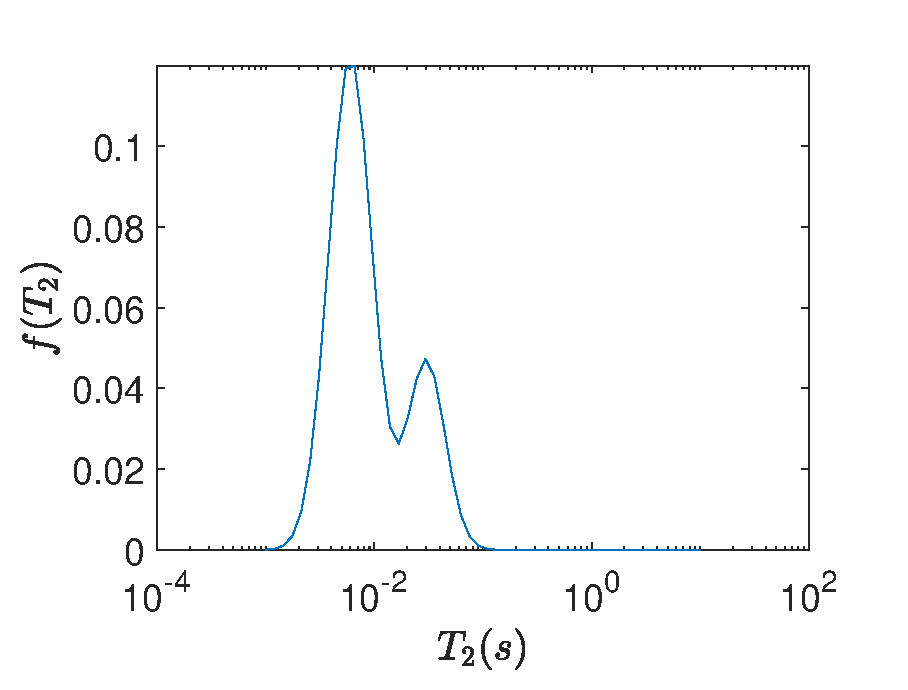
\includegraphics[width=\textwidth]{backgroundVector/densityFunction.eps}
        \subcaption{The density function $f(T_2)$}
        \label{fig:densityFunction}
    \end{subfigure}
    \begin{subfigure}[b]{0.495\textwidth}
        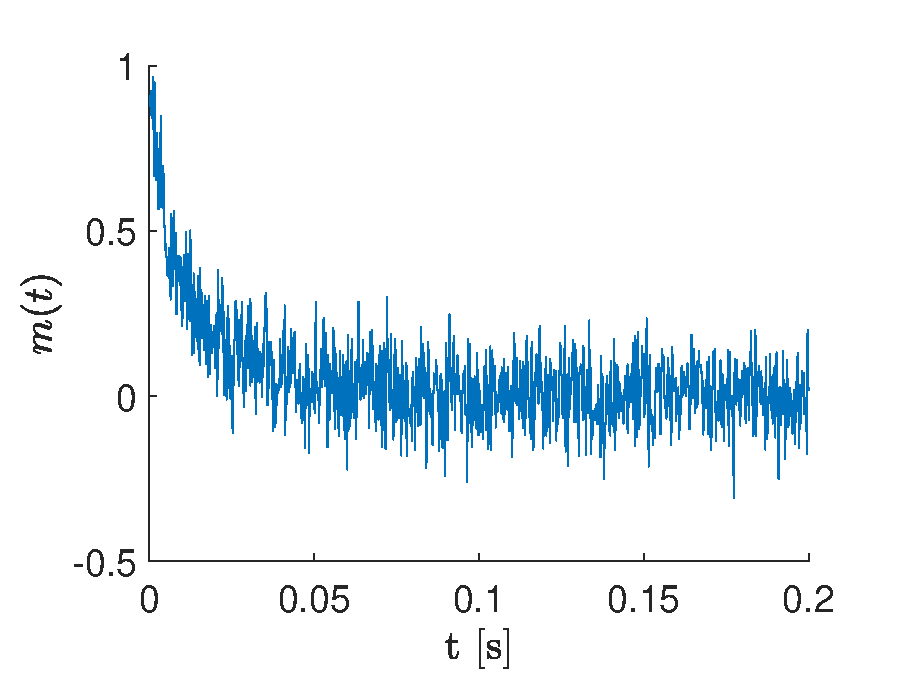
\includegraphics[width=\textwidth]{backgroundVector/measured.eps}
        \subcaption{The modelled measured data $m(t)$}
        \label{fig:measuredData}
    \end{subfigure}
    
    \caption{An example modelled $T_2$ density function and the measured data generated from it. It has unity porosity and a noise standard deviation of $\sigma_\epsilon = 0.2$}
    \label{fig:theModel}
\end{figure}

\subsubsection{Porosity}
The fraction of the rock volume that can be occupied by fluid is defined as the porosity ($\phi$) \cite{PorosityandT2Times}. After calibration with a water sample ($\phi = 1$), the integral over the entire density function is equal to the porosity.
\begin{equation}
    \phi = \int_0^\infty f(T_{2}) dT_{2}
\end{equation}
This is approximated to taking the sum over the discretised density function:
\begin{equation}
    \phi = \sum_i f(T_{2 i})
\end{equation}

\subsubsection{Bound Fluid Fraction}
Bound fluids are fluids that require significant capillary pressure to remove from porous media \cite{wellLoggingBook}. This pressure is caused by the fluid being placed in sufficiently small pores of the media. The volume of bound fluids - the bound fluid volume ($BFV$) \footnote{also known as the bulk fluid irreducible ($BVI$)} - is associated with relaxation times below a cut off value, $T_{2 \text{, cutoff}}$ \cite{wellLoggingBook}. This volume is obtained with:
\begin{equation}
    BFV = \int^{T_{2\text{, cutoff}}}_{T_{2\text{,min}}} f(T_2) d T_2
    \label{eq:boundFluidVolume}
\end{equation}
Free fluids conversely are fluids that are able to be extracted since they experience less capillary pressure restraining them \cite{NMRForRockskleinberg1993nuclear}\cite{BoundfluidFractionchen1998improving}. Therefore, the free fluid volume - also known as movable fluids ($BVM$) - can be expressed as the remaining fluid that is not bound in the T2 density function. Since the porosity is defined to be all of the fluid volume in the sample, the bound fluid fraction ($BFF$) can be expressed in terms of the porosity. 

The bound fluid fraction is expressed, where $T_{2\text{,min}} = 0$, as:
\begin{equation}
    BFF = 
    \frac{BFV}{BFV + BVM} =
    \frac{BFV}{\phi} = \frac{\int^{T_{2\text{, cutoff}}}_{0} f(T_2) d T_2}{\int_0^\infty f(T_{2}) dT_{2}}
    \label{eq:boundFluidFraction}
\end{equation}

\section{Inversion of Measured Data}
In order to compute the T2 relaxation times from the measured data we require a computational model that corroborates with the physical model. This model reveals that the measured data is ill-posed for an inversion problem.

\subsection{Model of T2 Relaxation Measurements}
The measured T2 relaxation of a sample can be modelled with the following integral
\begin{equation}
    m(t) = \int e^{\frac{-t}{T_2}} f(T_2) dT_2 + \epsilon
    \label{eq:T2RelaxationModelContinuous}
\end{equation}
As we are unable to numerically compute continuous functions, we discretise this into
\begin{equation}
    \hat{m}(t) = \sum^{N_y}_{k = 1} f_k e^{\frac{-t}{T_{2_k}}} + \epsilon
    \label{eq:T2RelaxationModel}
\end{equation}
This model corresponds with the detected exponential decay of the transverse magnetic field in eq. \ref{eq:T2ExpoenetialRelaxation}. The measurement data $m$ is made up of $N_2$ discrete measurements. The time constants of these exponential functions -$T_{2_k}$ - make up the T2 relaxation times. In the model itself: $N_y$ is the total number of relaxation times modelled, $f_k$ is the contribution of each exponential, and $\epsilon$ is the additive white Gaussian noise introduced by the measurement process.

Since we know the measurements are made of exponentially decaying functions, we can construct a kernel matrix, $K$, that maps from the T2 domain to the time domain. The T2 density function is modelled as a vector $f$. The measurement process is modelled by:
\begin{equation}
    m = Kf + \epsilon
    \label{eq:T2RelaxationModelMatrices}
\end{equation}


\subsection{Ill-posed Nature}
The goal of this project is to find the bound fluid fraction. This has traditionally required estimating $f$ and then computing from there. Transforming a \textit{noiseless} single exponential to an easily quantifiable time constant can be achieved with the Inverse Laplace Transform (ILT) \cite{BulterReedsDawsonMethod1981}.
\begin{equation}
   f_k\delta   \bigg(   \frac{1}{T_{2}} - \frac{1}{T_{2_k}} \bigg) = \mathcal{L}^{-1} \bigg\{ f_k e^{\frac{-t}{T_{2_k}}} \bigg\}
    \label{eq:InverseLaplaceNaive}
\end{equation}
The ILT is not suited for the noisy model due to the noise present in the measurements. There can be very different results for the same measured sample due to the random effect of noise. Also, the kernel matrix $K$ is very poorly conditioned for computation \cite{NumericalFredholm1971hanson1971numerical}. The measured signal cannot be frequency filtered since that process does not discriminate between the noise or the true signal. This necessitates the implementation of a numerical approximation of the inversion.

\section{The ILT (Inverse Laplace Transform) Technique}
The numerical inversion is based on the goal of minimising the difference between the true unknown distribution and the estimated distribution. The most popular technique is that described by Venkataramanan et al for one dimensional and two dimensional distributions \cite{Venk2DFredholm2002} \footnote{The ILT technique explored here is technically known as solving Fredholm integrals of the first kind}. This technique requires knowing the standard deviation of the noise present ($\sigma_\epsilon$).


\subsection{Inversion With Optimisation}
The Bulter-Reeds-Dawson (BRD) method \cite{BulterReedsDawsonMethod1981} provides the established technique for numerical computation of the ILT. This is an optimisation framework expressed as:
    
\begin{equation}
    \Phi(f) = \min_{f\geq0}  ||Kf_\alpha - m||^2 + \alpha||f_{\alpha}||^2
    \label{eq:minimseError1981Optimise}
\end{equation}    
In this framework we can see that the main cost being minimised is the difference between the hypothesised noiseless time domain data $Kf_\alpha$ and the actual measured data $m$. However, constricting the problem simply to just this allows for overfitting to the noise itself. To counteract this, the second term $\alpha||f_{\alpha}||^2$ is added to penalise the complexity of the hypothesised solution. This `smooths' the hypothesised $f$ to prevent it fitting to the noise \cite{RegularizationElden1977algorithms}. This process is known as \textit{regularisation}.
The BRD method \cite{BulterReedsDawsonMethod1981} sets the optimal regularisation parameter as
\begin{equation}
    \alpha_{\text{opt}} =  \frac{N_y \sqrt{ \sigma_{\epsilon} } }{||c||} 
    \text{, }
    \label{eq:optAlphaOptimise}
\end{equation} 
where the vector $c$ determines by the estimated density function $f_\alpha$ \cite{Venk2DFredholm2002} such that
\begin{equation}
    c =\frac {Kf_{\alpha} - m}{-\alpha}  
    \label{eq:optCOptimise}
\end{equation}  
    This method involves updating $c$ with $\alpha_{\text{opt}}$ and then computing $\alpha_{\text{opt}}$ for the new $c$ (fig. \ref{fig:2002Optimisation}). This iterative computation converges towards the density function we are trying to predict after approximately 20 iterations. The problem is convex \cite{BulterReedsDawsonMethod1981}, so the starting $\alpha$ and $c$ can be set to any value as it will automatically converge to the best answer. 

\begin{figure}[ht!]
    \centering
    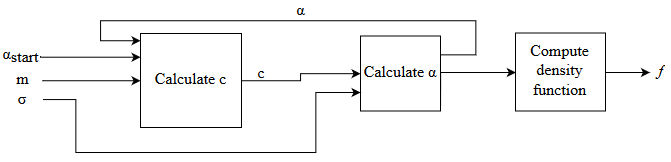
\includegraphics[width=\textwidth]{BlockDiagram2002Optimisation.png}
    \caption{Computational work flow of the optimisation framework in the inverse Laplace transform}
    \label{fig:2002Optimisation}
\end{figure}

\subsection{Calculating $c$}
    Computing the $c$ vector can be computationally dangerous due to potential error introduced by the approximate inversion of a possibly ill behaved matrix \cite{BulterReedsDawsonMethod1981}. Therefore, computing the $c$ vector involves taking the dot product of $m$ with a positive semi-definite matrix 
 
\begin{equation}
    H = \text{step}(K'c)I \text{, where} \quad \text{step}(t) = 
    \begin{cases}
    1  & t \geq 0\\
    0  & t < 0
    \end{cases}
    \label{eq:makeSemiPostiveDefinite}
\end{equation}   
that feeds in the regularisation coefficient \cite{BulterReedsDawsonMethod1981} $\alpha$ in the form of
\begin{equation}
    c =  (KHK' + \alpha I)^{-1} m  
    \label{eq:optFindC}
\end{equation} 


\subsection{Measurement Data Compression} \label{section:compression}
To reduce computation time, the truncated singular value decomposition of the kernel is used \cite{Venk2DFredholm2002}. Starting with the singular value decomposition $K = U S V'$:
\begin{itemize}
    \item the first $n$ columns $\hat{U}$ and $\hat{V}$ are kept from $U$ and $V$, and
    \item the first $n$ columns and rows of $\hat{S}$ are kept from S \cite{TSVDHansen1987truncatedsvd}.
\end{itemize}

\begin{equation}
    \hat{K} = \hat{S} \hat{V}'
    \label{eq:compressedKernel}
\end{equation}
\begin{equation}
    \hat{m} = m' \hat{U}
    \label{eq:compressedMeasurement}    
\end{equation}

These are then used to make a new kernel and measurement vector. Here, the dimensionality is reduced from $N_2$ (thousands) dimensions to $n$ dimensions   (eq. \ref{eq:compressedMeasurement}, \ref{eq:compressedKernel}). The optimisation problem remains unchanged as $||K||^2 = ||USV'||^2 \approx ||SV'||^2$; we are minimising the same error. This holds because the singular values of $K$ decay very rapidly as it is an exponential kernel \cite{NumericalInversionLaplaceTransform1978}.



\section{The ILT+ Technique}
More recent techniques have built further on this optimisation approach by implementing extra constraints. These come in the form of more prior information used to compensate for the high noise environment of the measured data \cite{GruberT2Estimation2013}. This involves calculating aspects that are intrinsic to the T2 density function. These are known as linear functionals. The two main functionals used for this improved optimisation framework are \textit{moments} and \textit{tapered areas} (fig. \ref{fig:2013ILTXOptimisation}) \cite{GruberT2Estimation2013}.


\begin{figure}[ht!]
    \centering
    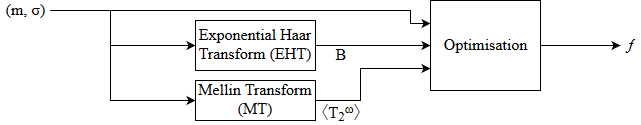
\includegraphics[width=0.9\textwidth]{ILTXBlockDiagram.png}
    \caption{Computational work flow of the optimisation framework for the ILT+ method.}
    \label{fig:2013ILTXOptimisation}
\end{figure}

\subsection{Estimation of Moments}
A moment is a description of the `weight' of the density function on the T2 axis \cite{VenkMellin2010}. An example of a moment is the first moment, the mean. The $\omega^{\text{th}}$ moment is defined as:

\begin{equation}
    \langle T_2^{\omega}  \rangle \equiv
    \frac
    {\int_{0}^{\infty}  T_2^{\omega} f_{T_2}(T_2)dT_2}
    {\int_{0}^{\infty}  f_{T_2}(T_2)dT_2 }
    =     
    \frac
    {\int_{0}^{\infty}  T_2^{\omega} f_{T_2}(T_2)dT_2}
    {\phi}
    \label{eq:defnMoment}
\end{equation}
The ILT+ requires an estimation of the moment directly from the measured data without knowledge of the density function. This estimation is implemented using the Mellin transform (MT) \cite{VenkMellin2010}:

\begin{equation}
\langle \hat{T_2^{\omega}}  \rangle =
\begin{cases}
        \frac{-1}{\Gamma (\mu) \phi}
        \int_{0}^{\infty}t^{\omega -1}[M(t) - \phi]dt &
        \text{ $-1<\omega<0$,}\\
        1 & \text{ $\omega=0$,}\\
        \frac{1}{\Gamma (\mu) \phi}
        \int_{0}^{\infty}t^{\omega -1}M(t)dt &
        \text{ $\omega>0$,}\\
\end{cases}
\label{eq:mellinTransform}
\end{equation}

The computed moment is a numerical value describing the density function. This has a propagated uncertainty that can be used to evaluate how much we should depend on it for the optimisation framework.


\subsection{Estimation of Tapered Areas}
Tapered areas are weighted areas under a T2 distribution \cite{TaperedAreaskleinberg1997tapered}. This is another linear functional that can be directly estimated from the measured data \cite{GruberLinearFunctionals2013}.

Tapered areas are computed directly from a density function by the use of a tapered step function. The specific transform used by Gruber et al is the Exponential Haar Transform (EHT) \cite{GruberLinearFunctionals2013}. This is defined in the $T_2$ domain as:

\begin{equation}
    K_a(T_2, T_c) = \frac{C}{\gamma}\tanh(\alpha \gamma) 
    \label{eq:expHaarTransformT2}
\end{equation}
The EHT is also defined in the time domain as:
\begin{equation}
    k_a(t, T_c) = C(-1)^n e^{\beta t} \text{, } \quad 2n\alpha < t < 2(n+1)\alpha \text{,}   \quad n \in \mathbb{Z}
    \label{eq:expHaarTransformTime}
\end{equation}
The actual tapered area ($B$) and the estimated tapered area ($\hat{B}$) are computed with an inner product of the EHT kernel and the data for their respective domains:

\begin{equation}
   \label{eq:estTaperedAreas}
   B = K_a(T_2,T_c)f(T_2),  \quad \hat{B} = k_a(t, T_c)m(t)
\end{equation}
The transform in the $T_2$ domain is normalised so that $T_2 = T_c$, $K = 0.5$ \cite{GruberLinearFunctionals2013}. To meet this property, the constants are set to be:
\begin{equation}
    C = \frac{0.7213}{T_c} \text{, } \quad \alpha = (1.572)T_c \text{, } \quad
   \beta = \frac{0.4087}{T_c}  \text{, } \quad \gamma = \frac{1}{T_2} + \beta  
   \label{eq:haarTransformConstants}
\end{equation}



\subsection{Constrained Optimisation}
    Directly estimated linear functionals are introduced as extra optimisation constraints to evaluate the accuracy of the estimated density function \cite{GruberT2Estimation2013}. These estimated functionals are also more accurate than simply using the ILT method \cite{GruberLinearFunctionals2013}. Therefore, the additional prior information yields a more accurate estimation of the density function in a low SNR environment. This forms the basis for the ILT+ method \cite{GruberT2Estimation2013}. The optimisation framework that aims to minimise the cost $Q(f_\alpha)$ takes the form of:
\begin{equation}
    Q(f_\alpha) = \min_{f\geq0}  ||W(Lf_\alpha - g)||^2 + \alpha||f_\alpha||^2
    \label{eq:2013Optimise}    
\end{equation}
    This framework is adapted from the ILT method (eq. \ref{eq:minimseError1981Optimise}) by appending the estimations and uncertainties of the tapered areas and moments onto the framework \cite{GruberT2Estimation2013} such that:
 \begin{equation}
    g = 
    \begin{bmatrix}
    m  \\
    \langle T_2^{\omega_1} \rangle \\
    \vdots \\
    \langle T_2^{\omega_{N_{m}}} \rangle \\
    B_1 \\
    \vdots \\
    B_{N_{a}}
    \end{bmatrix}
    \text{, } \quad
    L = 
    \begin{bmatrix}
    K  \\
    \frac{1}{\phi}T_{2}^{\omega_1}\\
    \vdots \\
    \frac{1}{\phi}T_{2}^{\omega_{N_{m}}}\\    
    K_{a}(T_2,T_{c_{1}}) \\
    \vdots \\
    K_{a}(T_2,T_{c_{3}})     
    \end{bmatrix}
    \text{, } \quad
    W = 
    \begin{bmatrix}
    \frac{1}{\sigma_\epsilon}  \\
    \frac{1}{\sigma_{\omega_1}}  \\ 
    \vdots \\
    \frac{1}{\sigma_{\omega_{N_{m}}}} \\
    \frac{1}{\sigma_B}\\
    \vdots\\
    \frac{1}{\sigma_{B_{N_{a}}}}
    \end{bmatrix}
    I
    \label{eq:2013NewOptVectors}  
\end{equation}    

\paragraph{}
    The $g$ vector contains $N_{m}$ estimated moments and $N_{a}$ estimated tapered areas. The $L$ matrix maps from the T2 domain to the time domain: the estimated density function ($f$), estimated moments of $f$, and estimated tapered areas of $f$. The $W$ matrix is a diagonal matrix that changes the weight of each respective value of $g$ and $L$ with division by their respective uncertainty. Therefore, the larger weight value we have, the more certain we are that the estimation is correct. The $m$ vector is compressed via the methodology detailed in section \ref{section:compression}. The compression is to the same degree as the ILT method. 

\paragraph{}
This review details the main techniques in the literature. The following section evaluates these techniques to form the benchmark for the proposed technique.






\chapter{Work Done}\label{C:prog}
The project has made significant progress on the first aim of implementing and evaluating the competing techniques. This has created the benchmark to evaluate the proposed method.
\section{Implementation of the Competing Techniques}
At this current point the main methods in the literature for the estimation of T2 relaxation times in a low SNR environment have been implemented and evaluated. They have been programmed from scratch using \textit{MATLAB}. The work done has focused on implementing these techniques and evaluating their effectiveness. The density used to demonstrate these techniques is given in figure \ref{fig:densityFunction}.


\subsection{The ILT Method}
The ILT method forms the basis for the estimation of the density function. This has been coded up and forms the basis for the other techniques to be developed. An example of this algorithm's operation is demonstrated in figure \ref{fig:2002ILTSimulation}. Its accuracy is demonstrated in the following techniques as the baseline.

 \begin{figure}[ht!]
    \centering
    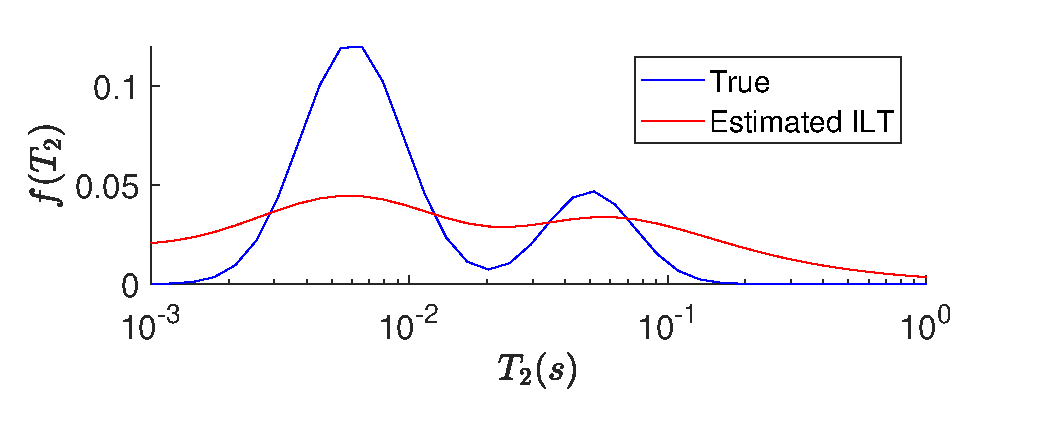
\includegraphics[width=0.6\textwidth]{backgroundVector/iltOptimise.eps}
    \caption{Application of the ILT inversion of measured data on the model.}
    \label{fig:2002ILTSimulation}
\end{figure}


\subsection{The Moment Estimator}
Evaluating the performance of the moment estimation involves comparing between the moments of the original density function, 
\begin{enumerate}
    \item the moments estimated with the Mellin transform, and
    \item the moments computed from the estimated distribution using the ILT.
\end{enumerate}
The accuracy of the moment estimator is measured using the normalised root mean square error ($NRMSE$) \cite{GruberT2Estimation2013} between the mean of the estimate and the true value.
\begin{equation}
    NRMSE = 100 \times
    \frac
    {\sqrt{(\mu_{\text{est}} - \mu_{\text{true}})^2}}
    {\mu_{\text{true}}}
    \label{eq:defnNRMSE}
\end{equation}

\begin{figure}[t]
    \centering
    \begin{subfigure}[b]{0.49\textwidth}
        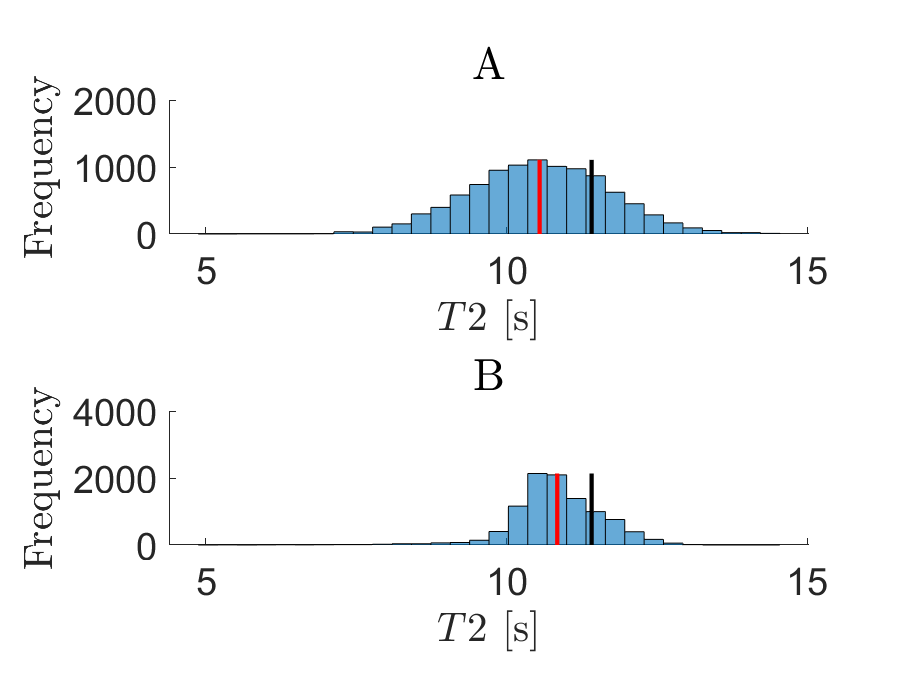
\includegraphics[width=\textwidth]{backgroundVector/moment-5e-1.eps}
        \subcaption{Estimation of the $-0.5^{th}$ moment of $f(T_2)$}
        \label{fig:moment5e-1Estimate}
    \end{subfigure}
    \begin{subfigure}[b]{0.49\textwidth}
        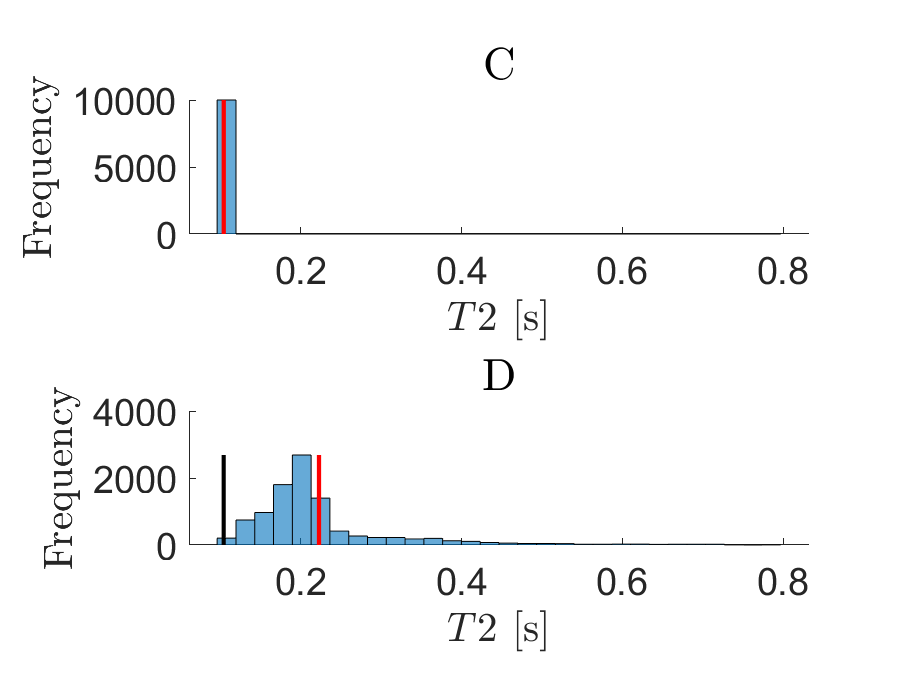
\includegraphics[width=\textwidth]{backgroundVector/moment5e-1.eps}
        \subcaption{Estimation of the $0.5^{th}$ moment of $f(T_2)$}
        \label{fig:moment1Estimate}
    \end{subfigure}
    
    \caption{The performance of the MT (A, C) compared to the ILT (B, D) in estimating the moments of the density function. Red is the mean of the estimated moment and black is the true moment.}
    \label{fig:estimateMoments}
\end{figure}
Figure \ref{fig:estimateMoments} demonstrates the performance of the Mellin transform versus the ILT for 10,000 different simulations. We see that the MT has a higher $NRMSE$ than the ILT for negative values of $\omega$. For higher values we see that the $NRMSE$ is significantly lower for the MT compared to the classic ILT.

\subsection {The Tapered Area Estimator}

Using the same methodology as moment estimation, the $NRMSE$ is used to quantify the accuracy of the EHT compared to the ILT (Fig. \ref{fig:estimateTaperedAreas}). We see that the EHT tapered area estimations have a significantly lower spread compared to the ILT. Furthermore, the $NRMSE$ of the EHT is typically smaller than the $NRMSE$ of the ILT method.

\begin{figure}
    \centering
    \begin{subfigure}[b]{0.49\textwidth}
        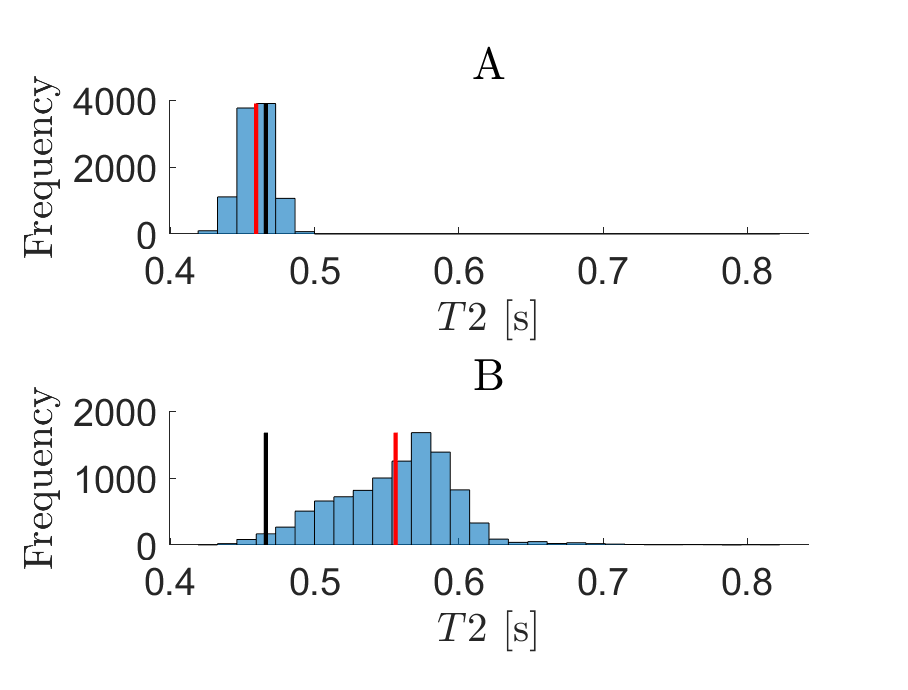
\includegraphics[width=\textwidth]{backgroundVector/area1e-2.eps}
        \subcaption{Estimation of the tapered area where $T_c = 0.01$ seconds}
        \label{fig:estTaperedAreaTc1e-1}
    \end{subfigure}
    \begin{subfigure}[b]{0.49\textwidth}
        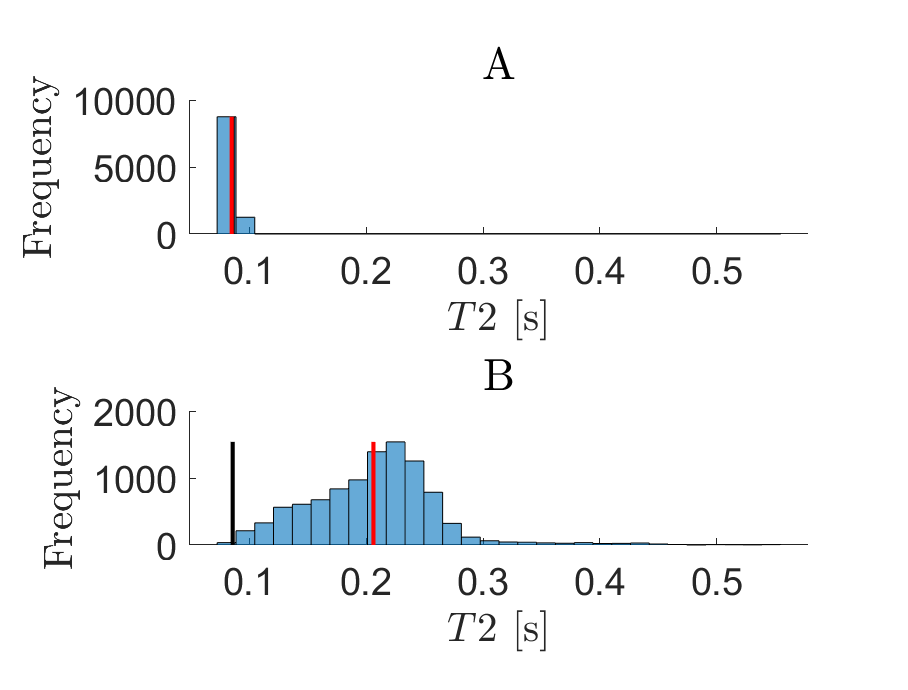
\includegraphics[width=\textwidth]{backgroundVector/area1e-1.eps}
        \subcaption{Estimation of the tapered area where $T_c = 0.1$ seconds}
        \label{fig:estTaperedAreaTc1}
    \end{subfigure}
    \caption{The performance of the EHT (A, C) compared to the ILT (B, D) in estimating the tapered area of the density function. Red is the mean of the estimated area and black is the true area.}
    \label{fig:estimateTaperedAreas}
\end{figure}


\subsection {The ILT+ Method}

The two metrics that were used to evaluate and compare this method with the ILT are:
\begin{itemize}
    \item the $NRMSE$ of the logarithmic mean ($T_{2_{LM}}$), and
    \item the $NRMSE$ of the bound fluid volume ($BFV$), with $T_c = 0.033 $s for sandstone \cite{TaperedAreaskleinberg1997tapered} \cite{wellLoggingBook}.
\end{itemize}

\paragraph{}
The use of linear functionals in the optimisation framework leads to more precise and accurate estimations of density function's properties \cite{GruberT2Estimation2013}. We see in figure \ref{fig:logMeanILT+} that the ILT+ method provides decreased bias and variance in predicting the logarithmic mean compared to the classic ILT. The error ($NRMSE$) is reduced with the introduction of linear functionals. Figure \ref{fig:BFVILT+} demonstrates that the ILT+ method also provides more accuracy and precision for predicting the bound fluid volume of a sample.

\begin{figure}[ht!]
    \centering
    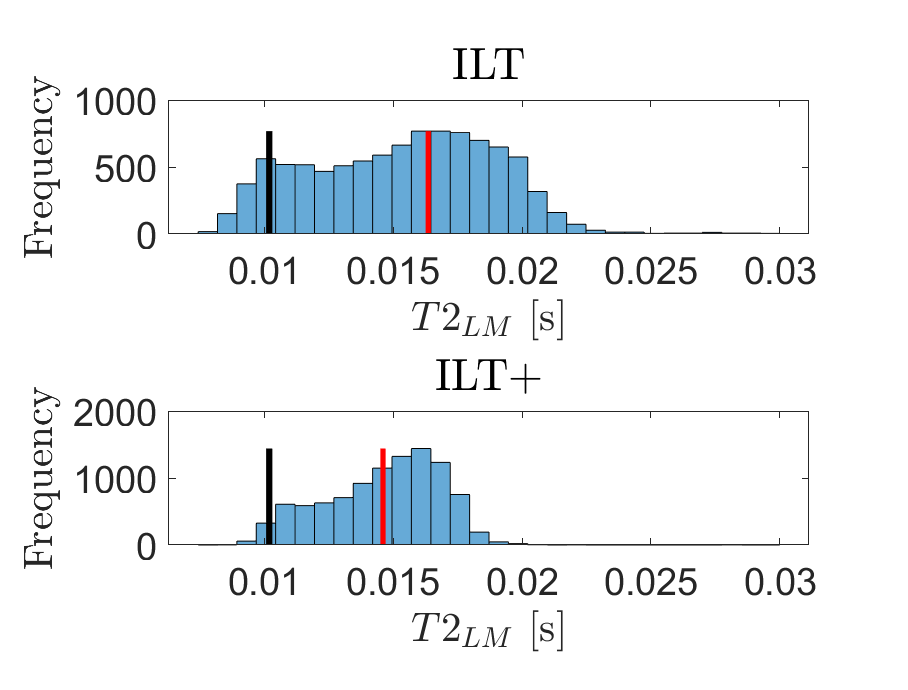
\includegraphics[width=0.5\textwidth]{backgroundVector/logMeanSimulate.eps}
    \caption{Estimation of the logarithmic mean directly from estimated distributions. Estimations by ILT and ILT+ are shown in plots A and B respectively. The black line is the true value and the red line is the estimated value.}
    \label{fig:logMeanILT+}
\end{figure}

\begin{figure}[ht!]
    \centering
    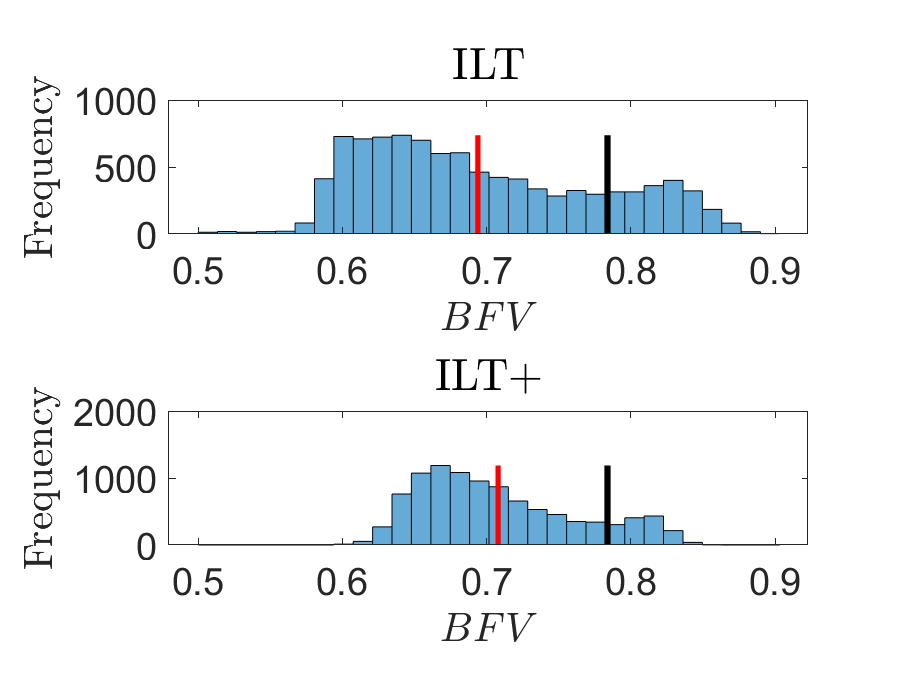
\includegraphics[width=0.5\textwidth]{backgroundVector/bfvSimulate.eps}
    \caption{Estimation of the bound fluid volume directly from estimated distributions. Estimations by ILT and ILT+ are shown in plots A and B respectively. The black line is the true value and the red line is the estimated value.}
    \label{fig:BFVILT+}
\end{figure}

These results make the ILT+ technique the benchmark to beat for this project`s proposed Bayesian method.
    
    
    











\chapter{Future Work}\label{C:prog}
The main constraint of the literature`s effectiveness has been on maintaining generality by constraining the amount of prior information that can be used. The future work seeks to allow for more reliable high quality experimental data to act as useful prior information. This introduces potential for more noise immunity in low SNR environments.

\section{Estimating Porosity}
Throughout the techniques explored the porosity was assumed to be already known and held constant. This is another linear functional that is solely dependent on measured data. That means it can be used to add another dimension onto the optimisation framework. Venkataramnan et al. have provided a method to estimate the porosity. This will be evaluated to allow for stronger evaluation of the current techniques available \cite{venkataramanan2015newPorosity}.

\section{Work on the New Bayesian Technique}
\subsection{Estimation of $f(T_2)$}
The Bayesian technique uses the probability of some measured data caused by a given density function to derive the likelihood of that function. This additional parameter allows for a more robust estimation. The starting point for this is detailed in \cite{paulTeal_NMRBayes}. The technique is expressed in Bayes' Rule as:
\begin{equation}
    p(f|m) = \frac{p(m|f)p(f)}{p(m)} = \frac{p(m|f)p(f)}{\int p(m|f)p(f) df}
    \label{eq:bayesMethod}
\end{equation}
where $f$ is a density function estimate, and $m$ is the measured data.

We can determine the best fitting $f$ by calculating and comparing $p(m|f)p(f)$ as $p(m)$ remains constant. Using the model expressed in equation \ref{eq:T2RelaxationModelMatrices}, the likelihood of measured data given a hypothesis takes the form of
\begin{equation}
    m|f \sim \mathcal{N}(Kf, C_\epsilon)
\end{equation}
where $C_\epsilon$ is the covariance of the noise.

\paragraph{}
The construction of the prior $p(f)$ in eq. \ref{eq:bayesMethod}, the likelihood of the density function, forms the crux of the technique. The development of the proposed technique will explore combining high quality laboratory data with low quality measured data to obtain $p(f)$. The integration of this into the pre-existing optimisation framework \cite{GruberT2Estimation2013} will be explored, implemented, and evaluated. Another possible technique of finding the optima of $p(f|m)$ for different $f$ will also be explored, implemented, and evaluated.

\subsection{Direct Estimation of $BBF$}
Bayes' Rule can also form the basis for estimating the bound fluid fraction directly with:
\begin{equation}
    p(BBF|m) = \frac{p(m|BBF)p(BBF)}{p(m)}
\end{equation}
The direct estimation of the bound fluid fraction is the overall goal of these estimation techniques so it will also be implemented and evaluated.

\section{Evaluation with Experimental Data}
There is a foundation to develop on top of the current optimisation framework to include high quality measured data. The high quality data to be used by the project is in the form of 30 experimental measurements of rock samples obtained from Schlumberger Doll Research. This allows for a stronger evaluation of the data to be made.
\\
Cross validation can be used to measure the accuracy of the estimation process \cite{crossValidation}. This involves splitting the dataset into three sets: the training set, test set, and validation set. The training dataset directly provides the algorithm information to calibrate it. The validation set evaluates the fitting of the trained estimator at each iteration. Finally, the test set evaluates the overall process. This final set prevents the tuning process from falling victim to overfitting or leaked information.


\section{Future Plan}
The future plan for the rest of the project is outlined in table \ref{tab:futurePlan}. Now that most of the current techniques have been recreated, construction can begin on the proposed method. Firstly, a simple version of the density function estimator will be constructed. It will grow in complexity for its second iteration with its integration of high quality experimental data. Afterwards, the estimator will augment the optimisation framework detailed in \cite{GruberT2Estimation2013}. Afterwards, a direct $BBF$ estimator will be explored. Finally, cross validation will implemented to evaluate the technique fairly.

\begin{table}[h]
    \centering
    \begin{tabular}{l l l}
        \toprule
        \hfill Task  &      Est. hours &     \hfill   Done by \\
        \midrule
        Improved porosity estimator \cite{venkataramanan2015newPorosity} & 20 & 22 June (Mid Exam Period) \\
        1st iteration $f(T_2)$ estimator & 25 & 6 July (End of Exam Period) \\
        Mid-project presentation & 10 & 13 July (Wk 1 Trimester 2)\\
        2nd iteration $f(T_2)$ estimator & 25 & 3 August (Wk 3 Trimester 2) \\
        New optimisation framework & 25 & 17 August (Wk 5 Trimester 2) \\
        $BBF$ estimator & 20 & 31 August (Wk 1 Mid-Trimester Break)\\
        Cross validation evaluation & 20 & 14 September (Wk 8 Trimester 2) \\
        Project snapshot completed & 5 & 1 October (Wk 10 Trimester 2)\\
        Writing the final report & 40 & 19 October (Wk 12 Trimester 2)\\
        \bottomrule
    \end{tabular}
    \caption{The future plan for the rest of the project}
    \label{tab:futurePlan}
\end{table}









\chapter{Conclusions}\label{C:con}
\paragraph{}
The current techniques for estimating the T2 density function and the bound fluid fraction have been constructed and evaluated. The estimation of linear functionals that describe the density function has been evaluated. The optimisation framework used to combine this prior information provides a foundation for the implementation and evaluation of high quality measurements with a Bayesian based methodology.
\paragraph{}
Evaluation of the estimation techniques have also been narrowed down to an easily comparable numerical value; the normalised root mean square error (NRMSE). The normalisation to percentage values allow for comparison between different distributions. This generality is important for assessing the applicability of this technique.
\paragraph{}
With these aspects implemented and considered, the project is ready to make effective progress into implementing the new Bayesian orientated technique. There is room for improvement for robustness and accuracy from the current ILT+ technique.

\section{Request for Feedback}
A significant number of the difficulties encountered involved programming up current methodology. Some of the issues are listed below
\begin{itemize}
    \item How to convincingly counteract over fitting since it is a major risk of the proposed technique?
    \item How necessary is it to report on the discrete versions of the Mellin transform and the Exponential Haar Transform that are used in the competing technique?
    \item This report has limited its analysis to one sample density function. To evaluate the final artefact, how many other density functions should be demonstrated in the final report?
    
\end{itemize}


%%%%%%%%%%%%%%%%%%%%%%%%%%%%%%%%%%%%%%%%%%%%%%%%%%%%%%%

\backmatter

%%%%%%%%%%%%%%%%%%%%%%%%%%%%%%%%%%%%%%%%%%%%%%%%%%%%%%%


\bibliographystyle{ieeetr}
%\bibliographystyle{acm}
\bibliography{sample}

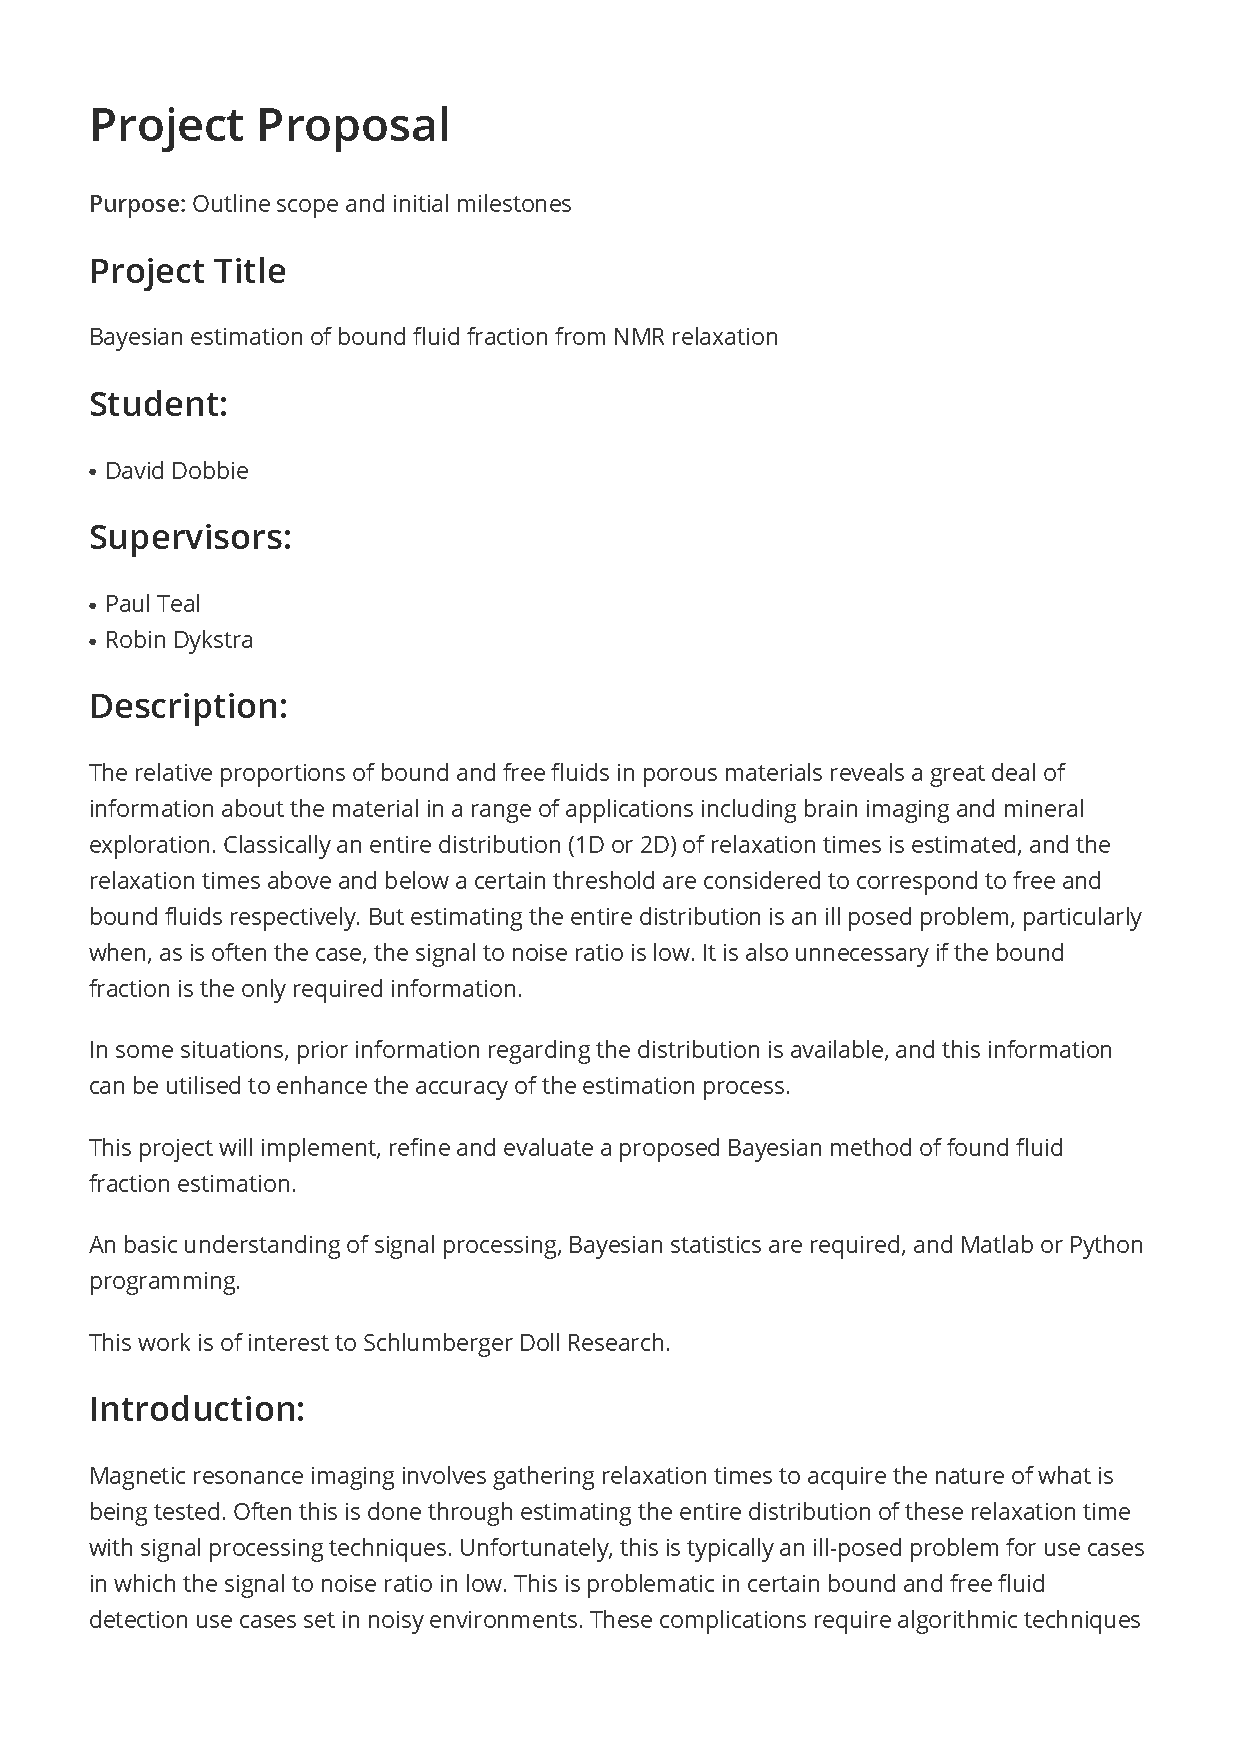
\includepdf[pages=-]{proposal.pdf}


\end{document}
